% =====================================================================
% Noise-Adaptive Patch-Based Image Restoration  (IEEE conference format)
% Structure follows the instructor's guide (Introduction, Literature Survey,
% Methodology, Results & Discussion incl. Dataset / Ablation / Quantitative /
% Qualitative, Failure Cases, Conclusion & Future Work).
% All numbers are produced from results/experiments/*.csv by
% analysis/make_tables.py (tables/*.tex are generated; do not edit by hand).
% Red \todo{...} marks must be resolved before submission.
% =====================================================================
\documentclass[conference]{IEEEtran}
\usepackage[T1]{fontenc}
\usepackage{amsmath,amssymb}
\usepackage{graphicx,xcolor}
\usepackage{booktabs,array}
\usepackage{tikz}
\usetikzlibrary{positioning,arrows.meta,fit,backgrounds}
\usepackage{pgfplots}
\pgfplotsset{compat=1.16}
\usepackage{cite}
\usepackage[hidelinks]{hyperref}

\newcommand{\todo}[1]{\textcolor{red}{\textbf{[#1]}}}
\newcommand{\figorbox}[3]{%
  \IfFileExists{#1}{\includegraphics[width=#2]{#1}}{%
  \fbox{\parbox[c][2.4cm][c]{\dimexpr#2-2\fboxsep-2\fboxrule}{\centering\footnotesize\textit{#3}\\[2pt](add \texttt{#1})}}}}
\newcommand{\PSNR}{\mathrm{PSNR}}
\newcommand{\MSE}{\mathrm{MSE}}

\begin{document}
\title{A Noise-Adaptive Patch-Based Image Restoration Pipeline:\\
Overlap-Weighted Reconstruction, Boundary Behaviour and Cost}

\author{\IEEEauthorblockN{Bandi Navadeep\IEEEauthorrefmark{1},
Rajan\IEEEauthorrefmark{2}, and Rohit\IEEEauthorrefmark{3}}
\IEEEauthorblockA{Department of Artificial Intelligence and Data Science\\
Indian Institute of Information Technology Raichur, Karnataka, India\\
\IEEEauthorrefmark{1}AD24B1014, \IEEEauthorrefmark{2}AD24B1051, \IEEEauthorrefmark{3}AD24B1053}}
\maketitle

\begin{abstract}
Convolutional denoisers are applied to high-resolution images patch by patch, but independently restored tiles can show seams and each noise type calls for a different model. We study a noise-adaptive pipeline that couples a multi-label noise detector with noise-specific DnCNN denoisers and weighted overlap-add reconstruction. Five controlled experiments on the first 20 DIV2K validation images, corrupted by Gaussian, salt-and-pepper and speckle noise at three severities (180 cases), isolate the effect of each component. Hann-weighted overlap-add at 25\% overlap improves PSNR by 0.26~dB (95\% CI 0.23--0.29) over non-overlapping tiling, and the gain is positive in all 180 cases; it also beats uniform blending by 0.074~dB. Beyond 25\% overlap the gain is indistinguishable from zero (+0.0003~dB) while inference time rises $2.1\times$. The detector classifies all 180 cases exactly, and routing costs +0.34~s (+43\%) with no loss in quality relative to known-noise selection. The pipeline raises mean PSNR from 21.32 to 37.03~dB, yet fails to improve severity-specific shallow CNNs at low noise (43 of 180 cases get worse). Results hold for synthetic single-noise corruption only.
\end{abstract}
\begin{IEEEkeywords}
image denoising, DnCNN, noise detection, patch-based inference, overlap-add, Hann window, PSNR, SSIM
\end{IEEEkeywords}

%=====================================================================
\section{Introduction}
\subsection{Background and Motivation}
Noise enters images through sensors, low light, transmission and processing, and its statistics differ by source: Gaussian noise is additive, salt-and-pepper noise replaces isolated pixels by extreme values, and speckle noise is multiplicative. Residual-learning CNNs such as DnCNN~\cite{zhang2017dncnn} remove a specified noise very effectively, but a model matched to one noise type is a poor match for another. This motivates detecting the noise type first and routing the image to the matching denoiser.

\subsection{Problem Statement and Limitations of Existing Approaches}
High-resolution images cannot always be restored in one pass, so they are processed in tiles. The SwinIR authors note that border pixels of a tile cannot use neighbours outside it, that tiles may therefore show border artefacts, and that overlapping patches reduce this at extra computational cost~\cite{liang2021swinir}. Overlapping tiles with window-weighted blending is an old idea in signal processing~\cite{allen1977} and segmentation~\cite{ronneberger2015unet}, yet recent restoration papers~\cite{zamir2022restormer,chen2022nafnet,potlapalli2023promptir,guo2024mambair} report the quality of the network and rarely the system-level cost of tiling. Three questions stay open for a practical pipeline: how much overlap and which blending weights are worth their cost, whether tile boundaries are measurably worse than tile interiors, and what an explicit noise detector adds to end-to-end latency.

\emph{Research question:} can a noise-adaptive pipeline with weighted patch reconstruction improve full-resolution quality at a practical computational cost?

\subsection{Objectives, Hypotheses and Contributions}
\textbf{Objectives.} (O1) Evaluate multi-label noise detection. (O2) Compare no-overlap, uniform and Hann-weighted reconstruction. (O3) Compare boundary and interior quality. (O4) Relate overlap to quality and time. (O5) Measure quality and cost of each model and of the full pipeline.

\textbf{Hypotheses.} \textbf{H1:} Hann-weighted overlap-add raises PSNR and SSIM over non-overlapping tiling. \textbf{H2:} Quality gains from overlap saturate while time keeps growing. \textbf{H3:} Detector-driven routing selects the correct denoiser, so the automatic pipeline matches known-noise selection in quality.

\textbf{Contributions.} (1) A paired, statistically quantified ablation of tiling, blending and routing on 180 cases. (2) A boundary/interior analysis with masks built from the real patch grid. (3) A per-noise, per-severity analysis including failure cases. (4) Documentation of the training protocol and a script-generated, reproducible results pipeline. Hann blending is an established operator and is evaluated here, not proposed as new.

%=====================================================================
\section{Literature Survey}
We review work from 2021--2026 on image restoration, with DnCNN~\cite{zhang2017dncnn} as the foundation of our denoisers. Table~\ref{tab:lit} compares five highly cited methods.

\begin{table*}[!t]
\caption{Representative restoration studies. Performance is as reported in each original paper, under different protocols and not comparable with ours. \todo{re-verify the citation counts on Google Scholar on the submission date and cite the access date}}
\label{tab:lit}
\centering\footnotesize
\renewcommand{\arraystretch}{1.15}
\begin{tabular}{p{2.4cm}p{3.3cm}p{3.3cm}p{2.9cm}p{4.2cm}}
\toprule
\textbf{Author(s) \& year (citations)} & \textbf{Methodology} & \textbf{Reported performance} & \textbf{Dataset} & \textbf{Critical remarks}\\
\midrule
Liang et al.\ 2021, SwinIR~\cite{liang2021swinir} (7952) & Residual Swin-Transformer blocks, shifted-window attention & Colour denoising, CBSD68, $\sigma{=}50$: 28.56~dB & Train: DIV2K, Flickr2K, BSD500, WED; test: CBSD68, Kodak24, McMaster & Strong context modelling and heavier than DnCNN; discusses tile borders but gives no overlap/blending study\\
Zamir et al.\ 2022, Restormer~\cite{zamir2022restormer} (7047) & Multi-Dconv transposed attention, gated-Dconv feed-forward & Real denoising, SIDD: 40.02~dB & SIDD, DND (also deblurring, deraining) & Efficient at high resolution; evaluates the network, not tiling or blending\\
Chen et al.\ 2022, NAFNet~\cite{chen2022nafnet} (2661) & Simple baseline without nonlinear activations & SIDD: 40.30~dB & SIDD, GoPro & Shows that simple blocks suffice; no explicit degradation detection\\
Potlapalli et al.\ 2023, PromptIR~\cite{potlapalli2023promptir} (907) & Learned prompts condition one all-in-one network & BSD68, $\sigma{=}25$ (3-task): 31.31~dB & BSD400/WED train; BSD68 test; plus dehazing, deraining & Implicit degradation adaptation; our pipeline detects noise explicitly and routes\\
Guo et al.\ 2024, MambaIR~\cite{guo2024mambair} (1488) & State-space (Mamba) blocks with local enhancement & Gains over SwinIR-class baselines reported on SR/denoising benchmarks & Standard SR, denoising and JPEG benchmarks & Linear-complexity alternative; not studied under overlapping-tile inference\\
\bottomrule
\end{tabular}
\end{table*}
% NOTE: performance numbers above are the papers' headline results as recalled; re-check each against its source.

Two further studies bear directly on our setting. TLC~\cite{chu2022tlc} shows that restoration networks with global pooling behave differently at training patch size and at full-image test size, and removes the mismatch at test time without retraining. AirNet~\cite{li2022airnet} infers the corruption type with a learned encoder instead of an explicit label. Our detector is the explicit, label-level counterpart of this idea.

\textbf{Research gap.} Prior work optimises the network or adapts implicitly to degradations. For fixed noise-specific denoisers, it is not quantified how patch overlap and blending weights trade quality against latency, how tile boundaries differ from interiors, and what an explicit noise detector costs end to end. This paper measures these effects with paired statistics and makes no comparative claim against the networks above, which were not run under our protocol.

%=====================================================================
\section{Methodology}
\subsection{Pipeline Overview}
Fig.~\ref{fig:pipe} shows the pipeline. A multi-label detector estimates which noise families are present; only the corresponding DnCNNs run, in a fixed order, each through overlapping patch inference with weighted aggregation.

\begin{figure*}[!t]
\centering
\resizebox{0.97\textwidth}{!}{%
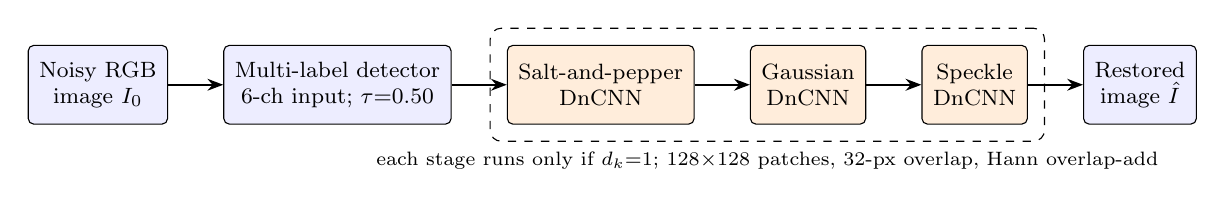
\begin{tikzpicture}[font=\footnotesize,node distance=7mm,
 blk/.style={draw,rounded corners=2pt,align=center,minimum height=10mm,fill=blue!7,inner sep=4pt},
 den/.style={blk,fill=orange!14},
 arr/.style={-{Stealth[length=2mm]},thick}]
\node[blk] (in) {Noisy RGB\\image $I_0$};
\node[blk,right=of in] (det) {Multi-label detector\\6-ch input; $\tau{=}0.50$};
\node[den,right=of det] (sp) {Salt-and-pepper\\DnCNN};
\node[den,right=of sp] (ga) {Gaussian\\DnCNN};
\node[den,right=of ga] (spk) {Speckle\\DnCNN};
\node[blk,right=of spk] (out) {Restored\\image $\hat I$};
\draw[arr] (in)--(det); \draw[arr] (det)--(sp); \draw[arr] (sp)--(ga);
\draw[arr] (ga)--(spk); \draw[arr] (spk)--(out);
\begin{pgfonlayer}{background}
\node[draw,dashed,rounded corners,fit=(sp)(ga)(spk),inner sep=6pt,
 label={[font=\scriptsize]below:{each stage runs only if $d_k{=}1$; $128{\times}128$ patches, 32-px overlap, Hann overlap-add}}] {};
\end{pgfonlayer}
\end{tikzpicture}}
\caption{Noise-adaptive restoration pipeline. Detector scores gate three noise-specific DnCNNs applied in the order salt-and-pepper, Gaussian, speckle.}
\label{fig:pipe}
\end{figure*}

\subsection{Multi-Label Noise Detector}
The input concatenates the RGB image with a high-pass view (image minus its $3{\times}3$ average-pooled version, scaled by four), giving six channels. Convolutional blocks of width 48, 96, 160 and 256 with max pooling are followed by global average and max pooling and a three-output linear head with logits $z_1,z_2,z_3$ for Gaussian, salt-and-pepper (SP) and speckle:
\begin{equation}
p_i=\frac{1}{1+e^{-z_i}},\qquad d_i=\mathbb 1[p_i\ge 0.50].
\end{equation}
For full images, $128{\times}128$ detector patches are processed without overlap, logits are averaged, then the sigmoid and threshold are applied.

\subsection{Noise-Specific Denoisers and Removal Order}
One DnCNN per family has 17 convolutional layers with 64 channels (Conv+ReLU, then Conv+BatchNorm+ReLU blocks, final 3-channel Conv). It predicts a residual: $\hat x=\mathrm{clip}(x-R_\theta(x),0,1)$. The baseline Basic CNN has four convolutions (3--32--64--32--3, ReLU, sigmoid output, no residual) and is trained per noise family \emph{and} severity (nine checkpoints). Selected denoisers run sequentially,
\begin{equation}
I_{k+1}=\begin{cases}F_k(I_k),&d_k=1\\ I_k,&d_k=0\end{cases},\qquad \mathcal O=[\text{SP},\text{Gauss},\text{Speckle}].
\end{equation}
The order is the reverse of the order in which the training code adds noise (speckle, then Gaussian, then SP), so each denoiser removes the noise that was added last. Its benefit on mixed noise was not tested.

\subsection{Training Protocol of the Checkpoints}
The project's shared training code (\texttt{common.py}) specifies: random $256{\times}256$ crops from a folder of clean images, a 70/15/15 train/validation/test split by source image (seed 42), random flips, and 8-bit quantisation after noising. Training strengths are drawn uniformly from $\sigma\in[5,60]/255$ (Gaussian), variance $[0.005,0.10]$ (speckle) and rate $[0.005,0.07]$ (SP); the test levels lie inside these ranges. Denoisers are trained with earlier-added noises present in the target with probability 0.5; the detector is trained on eight label subsets (clean, single, pairs, all three) with partially cleaned inputs produced by the real denoisers. The saved denoiser checkpoints store a validation PSNR of 30.34 (Gaussian), 46.23 (SP) and 33.01~dB (speckle). Optimizer, learning-rate schedule, epochs and loss are not recorded in the archive. \todo{state optimizer, epochs, learning rate, loss, and which images are in data/clean; confirm that none of DIV2K 0801--0820 is among them}

\subsection{Patch Extraction and Overlap-Weighted Reconstruction}
With patch size $P=128$ and overlap $o$, the stride is $s=P-o$; an extra final patch is aligned to the far edge when needed, and images smaller than a patch are replicate-padded. For patch predictions $\hat I_k$ and weights $W_k$,
\begin{equation}
\hat I(u,v)=\frac{\sum_k W_k(u,v)\,\hat I_k(u,v)}{\sum_k W_k(u,v)+\epsilon}.
\end{equation}
Uniform blending uses $W_k=1$. Hann blending uses the separable window
\begin{equation}
w(i)=\tfrac12\!\Big[1-\cos\tfrac{2\pi i}{P-1}\Big],\;\; W(i,j)=\tilde w(i)\tilde w(j),\;\; \tilde w=\max(w,0.05),
\end{equation}
so tile edges are down-weighted but never zero. The no-overlap configuration uses $o=0$.

\subsection{Metrics, Boundary Analysis and Statistics}
PSNR is $10\log_{10}(1/\MSE)$ for images in $[0,1]$; SSIM~\cite{wang2004ssim} uses data range 1.0 and a $7{\times}7$ window. The seam statistic is the mean absolute horizontal/vertical intensity difference in a 4-px mask around internal patch edges; it is a gradient measure, not an error against a seam-free reference. Boundary/interior PSNR uses an 8-px band around internal patch edges and reports $\Delta\PSNR=\PSNR_{\text{interior}}-\PSNR_{\text{boundary}}$.
Every comparison is \emph{paired}: both configurations see the same image, noise realisation and seed. We report the mean difference, a 95\% percentile bootstrap interval (5000 resamples), the share of cases improved, and a Wilcoxon signed-rank $p$-value. These describe variation over the 20 images $\times$ 9 noise settings only. Noise seeds are $42+100\cdot i+10\cdot j$ for image $i$ and severity $j$.

\subsection{Implementation}
PyTorch, NumPy, Pillow, OpenCV, scikit-image, pandas and psutil; CUDA inference in \texttt{eval()} and \texttt{inference\_mode()}; latency measured with warm-up and device synchronisation, one repeat per case. Checkpoint SHA-256 hashes are archived. \todo{insert GPU model, driver, CUDA and package versions}

%=====================================================================
\section{Results and Discussion}
\subsection{Dataset}
We use DIV2K~\cite{agustsson2017div2k}, a public benchmark of 2K-resolution images; the 100 validation images (0801--0900) are not used for training in the public protocol. Experiments 1--5 use the first 20 (0801--0820) at full resolution, mean about 2040$\times$1350 pixels, with the clean image as ground truth. Each is corrupted at three severities per family (Table~\ref{tab:cfg}), giving $20\times3\times3=180$ cases. A supplementary comparison of Basic CNN and DnCNN uses all 100 validation images resized to $128{\times}128$. No train/validation split is made in this study: it is an inference-only evaluation of the archived checkpoints (Section~III-D). Gaussian and speckle outputs are clipped and quantised to 8 bits; SP masks are shared across colour channels.

\begin{table}[!t]
\caption{Experimental configuration.}\label{tab:cfg}
\centering\footnotesize
\begin{tabular}{@{}ll@{}}
\toprule
Gaussian $\sigma$ & 10/255, 25/255, 50/255\\
Salt-and-pepper rate & 0.01, 0.03, 0.05\\
Speckle variance & 0.01, 0.04, 0.08\\
Images / cases & 20 / 180 (60 per family)\\
Patch size; overlaps & 128$\times$128; 0, 16, 32, 48, 64 px\\
Hann floor; detector $\tau$ & 0.05; 0.50\\
Seam / boundary mask & 4 px / 8 px\\
Timing & warm-up; 1 timed repeat per case\\
\bottomrule
\end{tabular}
\end{table}

\subsection{Ablation Study}
We add one component at a time on identical data and metrics (Table~\ref{tab:abl}). The Basic CNN row uses the same Hann 25\% reconstruction as the final system, so rows A and D differ only in the model.

\begin{table}[!t]
\caption{Ablation (means over 180 cases). Noise type is known except in E.}\label{tab:abl}
\centering\footnotesize
\setlength{\tabcolsep}{3pt}
\begin{tabular}{@{}clccccc@{}}
\toprule
 & Model + reconstruction & PSNR (dB) & SSIM & $\Delta$PSNR & Time (s)\\
\midrule
A & Basic CNN, Hann 25\% & 24.6125 & 0.7466 & --- & 0.247\\
B & DnCNN, no overlap & 36.7670 & 0.8945 & --- & 0.463\\
C & B + uniform 25\% overlap & 36.9545 & 0.8972 & +0.187 & 0.785\\
D & B + Hann 25\% overlap & \textbf{37.0285} & \textbf{0.8987} & +0.262 & 0.792\\
E & D + noise detector (auto) & \textbf{37.0285} & \textbf{0.8987} & 0.000 & 1.130\\
\bottomrule
\end{tabular}
\end{table}

\textbf{Blending and overlap.} Table~\ref{tab:stats} gives the paired comparisons. Hann 25\% improves PSNR over no overlap in 180 of 180 cases and over uniform blending in 99\% of cases; the seam statistic also falls (0.0280 $\to$ 0.0261 $\to$ 0.0257 for no overlap, uniform, Hann). Most of the gain arrives by 12.5\% overlap. From 25\% to 37.5\% or 50\% the interval includes zero or is at most 0.0007~dB, while the number of patches grows from 305 to 660 and time from 0.79~s to 1.69~s ($2.1\times$; Fig.~\ref{fig:sweep}). Overlap of 25\% is therefore a practical operating point for this setup, not a universal optimum. Gains from Hann blending vary by noise type: largest for SP (+0.36 to +0.56~dB over no overlap) and smallest for speckle (+0.11 to +0.14~dB), see Table~\ref{tab:sev}.

\begin{table}[!t]
\caption{Paired comparisons over 180 cases: mean $\Delta$PSNR (dB), 95\% bootstrap CI, share of cases improved, Wilcoxon $p$, mean $\Delta$SSIM.}\label{tab:stats}
\centering\scriptsize
\setlength{\tabcolsep}{2.5pt}
\begin{tabular}{@{}lccccc@{}}
\toprule
Comparison & $\Delta$PSNR & 95\% CI & Better & $p$ & $\Delta$SSIM\\
\midrule
Uniform 25\% vs.\ no overlap & +0.1874 & [+0.1691, +0.2078] & 100\% & $<10^{-6}$ & +0.0027\\
Hann 25\% vs.\ uniform 25\% & +0.0741 & [+0.0666, +0.0818] & 99\% & $<10^{-6}$ & +0.0016\\
Hann 25\% vs.\ no overlap & +0.2615 & [+0.2347, +0.2882] & 100\% & $<10^{-6}$ & +0.0042\\
12.5\% vs.\ 0\% overlap & +0.2421 & [+0.2177, +0.2683] & 100\% & $<10^{-6}$ & +0.0037\\
25\% vs.\ 12.5\% overlap & +0.0194 & [+0.0169, +0.0221] & 97\% & $<10^{-6}$ & +0.0005\\
37.5\% vs.\ 25\% overlap & +0.0002 & [-0.0002, +0.0005] & 52\% & 0.373 & +0.0000\\
50\% vs.\ 25\% overlap & +0.0003 & [-0.0000, +0.0007] & 58\% & 0.025 & +0.0000\\
\bottomrule

\end{tabular}
\end{table}

\begin{figure*}[!t]
\centering
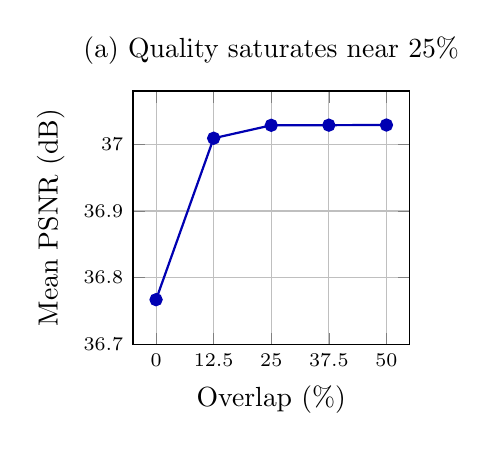
\begin{tikzpicture}
\begin{axis}[width=0.42\textwidth,height=4.8cm,xlabel={Overlap (\%)},ylabel={Mean PSNR (dB)},
 xtick={0,12.5,25,37.5,50},ymin=36.7,ymax=37.08,grid=major,tick label style={font=\scriptsize},
 title={(a) Quality saturates near 25\%}]
\addplot[mark=*,thick,blue!70!black] coordinates {(0,36.7670)(12.5,37.0091)(25,37.0285)(37.5,37.0287)(50,37.0289)};
\end{axis}
\end{tikzpicture}\hfill
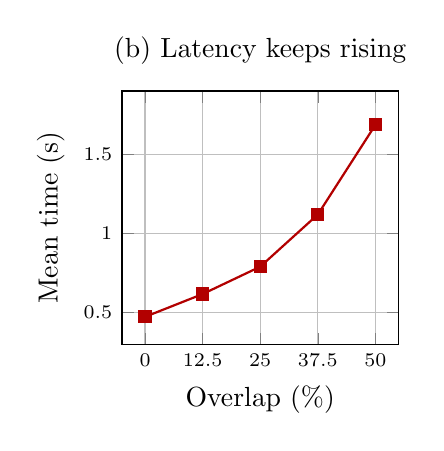
\begin{tikzpicture}
\begin{axis}[width=0.42\textwidth,height=4.8cm,xlabel={Overlap (\%)},ylabel={Mean time (s)},
 xtick={0,12.5,25,37.5,50},ymin=0.3,ymax=1.9,grid=major,tick label style={font=\scriptsize},
 title={(b) Latency keeps rising}]
\addplot[mark=square*,thick,red!70!black] coordinates {(0,0.4737)(12.5,0.6177)(25,0.7905)(37.5,1.1199)(50,1.6860)};
\end{axis}
\end{tikzpicture}
\caption{Overlap sweep (Exp.~3, Hann blending). Mean patches per image: 179, 238, 305, 435, 660.}
\label{fig:sweep}
\end{figure*}

\textbf{Boundary versus interior (Exp.~2).} At 32-px overlap, interior PSNR exceeds boundary PSNR on average by 0.085~dB (95\% CI 0.066--0.105; positive in 72\% of cases): Gaussian +0.070 [0.047, 0.095], SP +0.050 [0.012, 0.090], speckle +0.136 [0.102, 0.170]. The effect is real but small. SSIM differences are tiny (mean $-0.0007$, mixed sign by family), so there is a modest PSNR boundary gap, not a general seam penalty.

\subsection{Quantitative Analysis}
Table~\ref{tab:sev} breaks the full pipeline down by noise family and severity. PSNR gain grows with severity for Gaussian (+6.4, +10.3, +11.7~dB) and speckle, and is large for SP at all levels (about +26~dB). Gaussian is the weakest family in absolute quality (26.8~dB at $\sigma{=}50$). Overall, mean PSNR rises from 21.32 to 37.03~dB (+15.71~dB) and mean SSIM from 0.482 to 0.899.

\begin{table*}[!t]
\caption{Pipeline results by noise family and severity (means over 20 images). ``Basic gain'' is the Basic CNN's PSNR gain over the noisy input; ``Hann gain'' is Hann 25\% over no overlap.}\label{tab:sev}
\centering\footnotesize
\begin{tabular}{@{}llcccccc@{}}
\toprule
Noise & Severity & Noisy PSNR & Restored PSNR & Gain (dB) & SSIM & Basic gain (dB) & Hann gain (dB)\\
\midrule
Gaussian & Low & 28.29 & 34.67 & +6.38 & 0.911 & -2.44 & +0.250\\
 & Medium & 20.57 & 30.83 & +10.26 & 0.829 & +4.02 & +0.220\\
 & High & 15.07 & 26.81 & +11.73 & 0.660 & +7.96 & +0.180\\
\midrule
Salt-pepper & Low & 24.88 & 51.54 & +26.66 & 0.998 & +0.42 & +0.560\\
 & Medium & 20.11 & 46.60 & +26.49 & 0.994 & +4.88 & +0.409\\
 & High & 17.90 & 43.83 & +25.93 & 0.989 & +6.00 & +0.357\\
\midrule
Speckle & Low & 26.41 & 35.74 & +9.33 & 0.944 & -1.06 & +0.109\\
 & Medium & 20.70 & 32.52 & +11.82 & 0.901 & +3.92 & +0.125\\
 & High & 17.91 & 30.72 & +12.81 & 0.863 & +5.96 & +0.144\\
\bottomrule

\end{tabular}
\end{table*}

\textbf{Model comparison and cost.} The Basic CNN is the fastest (0.25~s, 4.1 img/s) but 12.4~dB below DnCNN; it is trained separately for every severity and still lowers PSNR at low noise. On all 100 validation images at $128{\times}128$ the same pattern holds (Table~\ref{tab:all}): DnCNN improves PSNR by +12.7~dB on average against +2.1~dB for the Basic CNN. Fig.~\ref{fig:qlat} shows the quality--latency trade-off of Table~\ref{tab:abl}. Adding the detector costs 0.34~s per image (95\% CI 0.31--0.36; +43\%) and leaves PSNR and SSIM identical in all 180 cases.

\begin{table}[!t]
\caption{Basic CNN (severity-specific) vs.\ DnCNN on all 100 validation images, $128{\times}128$.}\label{tab:all}
\centering\scriptsize
\setlength{\tabcolsep}{2.5pt}
\begin{tabular}{@{}llccccc@{}}
\toprule
Noise & Level & Noisy & \multicolumn{2}{c}{PSNR (dB)} & \multicolumn{2}{c}{SSIM}\\
 & & PSNR & Basic & DnCNN & Basic & DnCNN\\
\midrule
Gaussian & Low & 28.27 & 24.39 & 32.39 & 0.846 & 0.934\\
 & Medium & 20.58 & 23.65 & 28.27 & 0.778 & 0.863\\
 & High & 15.10 & 22.33 & 24.81 & 0.686 & 0.727\\
\midrule
Salt-pepper & Low & 24.90 & 24.26 & 47.92 & 0.819 & 0.998\\
 & Medium & 20.12 & 23.67 & 42.97 & 0.755 & 0.996\\
 & High & 17.88 & 22.89 & 40.39 & 0.724 & 0.992\\
\midrule
Speckle & Low & 27.14 & 24.40 & 33.18 & 0.825 & 0.957\\
 & Medium & 21.38 & 23.72 & 29.81 & 0.782 & 0.917\\
 & High & 18.56 & 23.25 & 28.07 & 0.751 & 0.882\\
\bottomrule

\end{tabular}
\end{table}

\begin{figure}[!t]
\centering
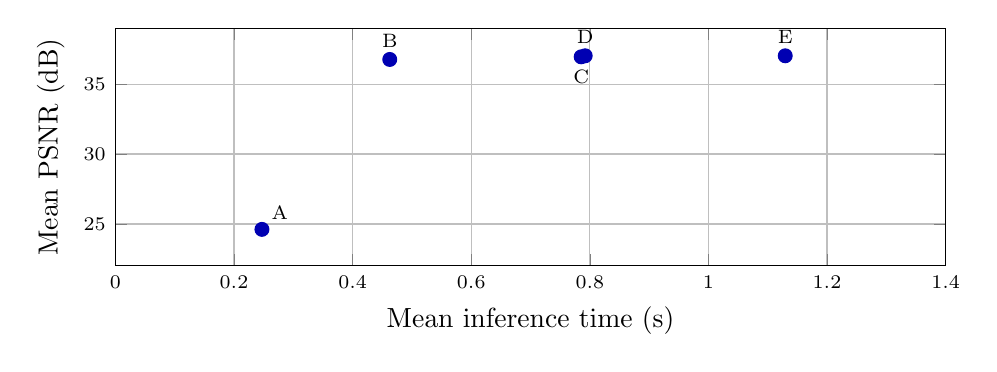
\begin{tikzpicture}
\begin{axis}[width=\columnwidth,height=4.6cm,xlabel={Mean inference time (s)},ylabel={Mean PSNR (dB)},
 xmin=0,xmax=1.4,ymin=22,ymax=39,grid=major,tick label style={font=\scriptsize}]
\addplot[only marks,mark=*,mark size=2.5pt,blue!70!black] coordinates {(0.2471,24.6125)(0.4626,36.7670)(0.7854,36.9545)(0.7922,37.0285)(1.1295,37.0285)};
\node[above right,font=\scriptsize] at (axis cs:0.2471,24.6) {A};
\node[above,font=\scriptsize] at (axis cs:0.4626,36.9) {B};
\node[below,font=\scriptsize] at (axis cs:0.7854,36.7) {C};
\node[above,font=\scriptsize] at (axis cs:0.7922,37.2) {D};
\node[above,font=\scriptsize] at (axis cs:1.1295,37.2) {E};
\end{axis}
\end{tikzpicture}
\caption{Quality--latency trade-off (labels as in Table~\ref{tab:abl}).}
\label{fig:qlat}
\end{figure}

\textbf{Noise detection (Exp.~5).} Each label is evaluated on 60 positive and 120 negative cases. Precision, recall, F1 and accuracy are 1.00 for all three labels (180 of 180 exact matches; Table~\ref{tab:conf}). The weakest decision margins are a lowest positive score of 0.994 (speckle) and a highest negative score of 0.167 (speckle), so the 0.50 threshold is not close to being crossed. This is a single-noise synthetic test and does not show robustness to mixed or real noise.

\begin{table}[!t]
\caption{Detector confusion matrix (counts; columns: predicted).}\label{tab:conf}
\centering\footnotesize
\begin{tabular}{@{}lcccc@{}}
\toprule
True $\backslash$ pred. & Gaussian & SP & Speckle & None\\
\midrule
Gaussian & 60 & 0 & 0 & 0\\
Salt-and-pepper & 0 & 60 & 0 & 0\\
Speckle & 0 & 0 & 60 & 0\\
\bottomrule
\end{tabular}
\end{table}

\subsection{Qualitative Analysis}
Fig.~\ref{fig:qual} shows the boundary and interior masks on image 0801 and a Gaussian-denoising comparison on validation image 0874 (outside the 20-image subset). The Basic CNN output retains visible blotchy residual noise and colour shifts that the DnCNN output removes, which matches the 12~dB gap in Table~\ref{tab:abl}. Aggregate metrics do not show where residual artefacts sit; zoomed seam crops with error maps for all three blending modes are listed as future work.

\begin{figure}[!t]
\centering
\figorbox{fig/boundary-masks.png}{0.95\columnwidth}{clean / restored (Hann) / 8-px boundary mask / interior mask}\\[4pt]
\figorbox{fig/qualitative-0874.png}{0.95\columnwidth}{clean / noisy / Basic CNN / DnCNN (Gaussian)}
\caption{Top: clean image, Hann-restored image, boundary and interior masks (image 0801). Bottom: original, noisy, Basic CNN and DnCNN outputs (image 0874).}
\label{fig:qual}
\end{figure}

\section{Failure Cases and Limitations}\label{sec:fail}
\textbf{Where the method performs poorly.}
(i) \emph{Strong Gaussian noise.} The five lowest restored PSNRs all belong to Gaussian cases at $\sigma\ge25/255$ (Table~\ref{tab:worst}), and the lowest SSIM values (0.55--0.59, images 0816, 0813, 0805) are Gaussian $\sigma{=}50/255$ cases.
(ii) \emph{One difficult image.} Image 0807 has a mean gain of only 8.8~dB against 15.7~dB overall (the next lowest image: 14.3~dB), and contains the single worst case (22.55~dB). We have not yet inspected this image, so the cause (for example fine texture) is unverified.
(iii) \emph{Basic CNN at low noise.} The severity-specific Basic CNN makes 43 of 180 cases worse than the noisy input (mean $-2.44$~dB for Gaussian low, $-1.06$~dB for speckle low).
(iv) \emph{Boundary gap and cost.} A small PSNR gap remains at tile boundaries (up to 0.14~dB), overlap above 25\% is pure cost, and detection adds 43\% latency.
\todo{run analysis/make\_failure\_figure.py, insert fig/failure-cases.png here and describe what the crops show for 0807}

\begin{table}[!t]
\caption{Five lowest restored-PSNR cases (Hann 25\%, automatic pipeline).}\label{tab:worst}
\centering\footnotesize
\begin{tabular}{@{}lllccc@{}}
\toprule
Image & Noise & Level & Noisy PSNR & Restored PSNR & SSIM\\
\midrule
0807 & Gaussian & High & 15.30 & 22.55 & 0.643\\
0804 & Gaussian & High & 15.03 & 25.65 & 0.640\\
0805 & Gaussian & High & 14.98 & 25.68 & 0.585\\
0807 & Gaussian & Medium & 20.78 & 25.70 & 0.796\\
0820 & Gaussian & High & 15.42 & 25.80 & 0.741\\
\bottomrule

\end{tabular}
\end{table}

\begin{figure}[!t]
\centering
\figorbox{fig/failure-cases.png}{0.95\columnwidth}{crops of the lowest-PSNR cases: clean / noisy / restored / error map}
\caption{Failure cases from the per-case analysis.}
\end{figure}

\textbf{Limitations.} Only 20 images (full resolution) and synthetic single-family noise; no mixed-noise, real-noise (SIDD, PolyU) or cross-dataset evaluation, so detector accuracy of 100\% says nothing about real images. Optimizer, schedule and epochs of the checkpoints are not recorded. Latency is a single timed run per case on unrecorded hardware, and each experiment was timed in its own pass, so absolute times differ slightly between tables (no-overlap: 0.52, 0.47, 0.46~s); compare within a table only. The seam statistic is a gradient measure and can reflect real image structure. No external baseline (SwinIR, Restormer, NAFNet, PromptIR, MambaIR) was run under matched conditions.

\section{Discussion}
\begin{table}[!t]
\caption{Hypotheses versus evidence.}\label{tab:hyp}
\centering\footnotesize
\begin{tabular}{@{}p{0.6cm}p{5.4cm}p{1.8cm}@{}}
\toprule
 & Evidence & Verdict\\
\midrule
H1 & Hann 25\%: +0.262~dB (CI 0.235--0.288), +0.0042 SSIM, better in 180/180 cases & Supported\\
H2 & 0$\to$12.5\%: +0.242~dB; 25$\to$50\%: +0.0003~dB (CI includes 0); time $2.1\times$ & Supported\\
H3 & 180/180 exact detection; auto = known-noise quality in every case & Supported (single noise)\\
\bottomrule
\end{tabular}
\end{table}
The effects of blending are statistically unambiguous but small in absolute terms: they matter when a system is already near its quality ceiling and cost is the constraint. The larger levers in this study are the model (+12.4~dB over the Basic CNN) and the noise severity. The detector is cheap relative to its benefit only when the noise type is genuinely unknown; its quality benefit over known-noise routing is zero by construction. Whether the reverse-order cascade works on mixed noise is untested, although the training code is built for it.

%=====================================================================
\section{Conclusion and Future Work}
We evaluated a noise-adaptive patch-based restoration pipeline with paired statistics on 180 synthetic cases from 20 DIV2K images. Hann-weighted overlap-add at 25\% overlap improves PSNR by 0.26~dB over non-overlapping tiling in every case, larger overlaps add cost without measurable gain, the detector is exact on single-noise cases and the full pipeline lifts mean PSNR by 15.7~dB at 0.34~s routing cost. H1--H3 are supported within this synthetic setting. Limits: small subset, synthetic single-family noise, single-run timing and incomplete training records.

\textbf{Future work:} (1) all 100 validation images, mixed-noise tests (the detector and cascade are built for them) and real-noise datasets such as SIDD and PolyU; (2) repeated timing with confidence intervals and recorded hardware; (3) zoomed seam crops, error maps and perceptual metrics such as LPIPS; (4) matched comparisons with SwinIR, Restormer or NAFNet and full training documentation; (5) batched patch inference and a lighter detector to cut the 43\% routing overhead.

\begin{thebibliography}{12}
\bibitem{zhang2017dncnn} K. Zhang, W. Zuo, Y. Chen, D. Meng, and L. Zhang, ``Beyond a Gaussian denoiser: Residual learning of deep CNN for image denoising,'' \emph{IEEE Trans. Image Process.}, vol. 26, no. 7, pp. 3142--3155, 2017.
\bibitem{liang2021swinir} J. Liang, J. Cao, G. Sun, K. Zhang, L. Van Gool, and R. Timofte, ``SwinIR: Image restoration using Swin Transformer,'' in \emph{Proc. ICCVW}, 2021, pp. 1833--1844.
\bibitem{zamir2022restormer} S. W. Zamir, A. Arora, S. Khan, M. Hayat, F. S. Khan, and M.-H. Yang, ``Restormer: Efficient Transformer for high-resolution image restoration,'' in \emph{Proc. CVPR}, 2022, pp. 5728--5739.
\bibitem{chen2022nafnet} L. Chen, X. Chu, X. Zhang, and J. Sun, ``Simple baselines for image restoration,'' in \emph{Proc. ECCV}, 2022, pp. 17--33.
\bibitem{potlapalli2023promptir} V. Potlapalli, S. W. Zamir, S. Khan, and F. S. Khan, ``PromptIR: Prompting for all-in-one image restoration,'' in \emph{Adv. Neural Inf. Process. Syst.}, vol. 36, 2023.
\bibitem{guo2024mambair} H. Guo, J. Li, T. Dai, Z. Ouyang, X. Ren, and S.-T. Xia, ``MambaIR: A simple baseline for image restoration with state-space model,'' in \emph{Proc. ECCV}, 2024.
\bibitem{chu2022tlc} X. Chu, L. Chen, C. Chen, and X. Lu, ``Improving image restoration by revisiting global information aggregation,'' in \emph{Proc. ECCV}, 2022.
\bibitem{li2022airnet} B. Li, X. Liu, P. Hu, Z. Wu, J. Lv, and X. Peng, ``All-in-one image restoration for unknown corruption,'' in \emph{Proc. CVPR}, 2022.
\bibitem{ronneberger2015unet} O. Ronneberger, P. Fischer, and T. Brox, ``U-Net: Convolutional networks for biomedical image segmentation,'' in \emph{Proc. MICCAI}, 2015, pp. 234--241.
\bibitem{allen1977} J. B. Allen, ``Short term spectral analysis, synthesis, and modification by discrete Fourier transform,'' \emph{IEEE Trans. Acoust., Speech, Signal Process.}, vol. 25, no. 3, pp. 235--238, 1977.
\bibitem{agustsson2017div2k} E. Agustsson and R. Timofte, ``NTIRE 2017 challenge on single image super-resolution: Dataset and study,'' in \emph{Proc. CVPRW}, 2017, pp. 126--135.
\bibitem{wang2004ssim} Z. Wang, A. C. Bovik, H. R. Sheikh, and E. P. Simoncelli, ``Image quality assessment: From error visibility to structural similarity,'' \emph{IEEE Trans. Image Process.}, vol. 13, no. 4, pp. 600--612, 2004.
\end{thebibliography}
\end{document}
